%\documentclass{article}
\documentclass[twocolumn]{article}
\usepackage[utf8]{inputenc}
\usepackage{tikz}
\usetikzlibrary{positioning,fit,shapes,arrows.meta}
\usepackage{hyperref}

\author{ K\'evin Le Bon \and Alan Schmitt }

\title{MLExplain}

\begin{document}
\maketitle

\begin{abstract}
  MLExplain is a step-by-step interpreter for OCaml that enables the
  user to inspect both their program's state and the interpreter's state
  itself. This interpreter aims to provide the user with a better understanding
  of the semantics of OCaml.
\end{abstract}

\section{Introduction}

The semantics of a programming language can be very complex. When a language
has no specification, the semantics is then defined by the implementations of
the language, i.e., interpreters and compilers. However even when a
specification is available, it can be difficult to understand why the execution
of a specific program results to a certain output.

The goal of the \emph{JSExplain} project \cite{chargueraud:hal-01745792} is to
describe the execution of a JavaScript program by showing every step of an
interpreter whose behavior is very close to the specification of JavaScript. In
this paper, we show how we adapted JSExplain to OCaml.

Unlike JavaScript, OCaml has no official specification. However, OCaml code
execution is fairly simple because the number of language constructions is
small. We have written an interpreter for OCaml's typed abstract syntax tree
(AST). This AST is still close to the source code yet it provides additional
crucial information. For instance, it mentions resolved names, which is useful
for module and signatures inclusion and mandatory for interpreting features like
named parameters and optional parameters in functions. The semantic we give to
OCaml is higher level than the one described in \emph{ZINC} \cite{Leroy-ZINC}
virtual machine, i.e., an interpreter for bytecode after compilation.

\section{JSExplain}

\subsection{A Double Debugger}
\label{subsec:double-debugger}

We call a \emph{double debugger} an interpreter that is able to run step by step
and display the program's state and current location in source, as well as the
state and location in the source of the interpreter itself. JSExplain is a
double debugger for JavaScript. The aim of this tool is to help a user to better
understand JavaScript's semantics, by providing an interpreter that is very
close to the specification of JavaScript. JSExplain's interface highlights the
expression of the program currently evaluated as well as the instruction of the
interpreter that is executed.

\subsection{Architecture}

The core of JSExplain is a JavaScript interpreter written in a subset of OCaml.
This interpreter is compiled to a subset of JavaScript and instrumented to
generate a trace of its execution when run. This trace can then be navigated
using a web-based
tool.\footnote{\url{https://jscert.github.io/jsexplain/branch/master/driver.html}}

The subset of OCaml we support for writing the interpreter is purely functional
with variables, constants, sequence, conditional, let-binding, function
definition, function application (with support for prefix and infix functions),
data constructors, records (including record projections, and the
``record-with'' construct to build a copy of a record with a number of fields
updated), tuples (i.e., anonymous records), and simple pattern matching (only
with non-nested patterns, restricted to data constructors, constants, variables,
and wildcards). For convenience, let-bindings and functions may bind simple
patterns (as opposed to only variables). We also support \texttt{ppx} extensions
for monadic programming, to simplify the handling of errors.

The target language of our compiler is a purely functional subset of JavaScript
where there is never any type conversion, where objects are used as records (no
use of their \texttt{prototype} field), and where tuples are encoded into
arrays.

We instrument the compilation to JavaScript by adding code that logs events,
namely entering a function, creating a scope, assigning a variable, and exiting
a function. Each event captures the state, the stack, and the values of all
local variables in scope of the interpreter code at the point where the event
gets triggered. Code that is traced is compiled with this instrumentation,
whereas code that is not traced, for instance supporting libraries, is directly
compiled to JavaScript.

When using the tool, the source JavaScript program is parsed and run through the
instrumented interpreter, thus generating a trace. We can then navigate this
trace to see the state of the interpreter as well as the state of the
interpreted program. Recovering the information about the interpreted code is
not completely straightforward. For example, to recover the fragment of code to
highlight, we find in the trace the closest previous event that contains a call
to function with an argument named \texttt{\_term\_}. This argument corresponds
to the AST of a subexpression, and this AST is decorated (by the parser) with
locations. Note that, for efficiency reasons, we associate to each event from
the trace its corresponding \texttt{\_term\_} argument during a single pass,
performed immediately after the trace is produced.

Similarly, we are able to recover the state and environment associated with the
event. The state of the interpreted program consists of four fields: the
strictness flag, the value of the \texttt{this} keyword, the lexical
environment, and the variable environment. We implemented a custom display for
these elements, and also for values of the languages, in particular for objects:
one may click on an object to reveal its contents and recursively explore it.

Finally, a web interface is presented to the user, to navigate in the trace.
This navigation can be forward and backward, and at all times the source code
and interpreter code are highlighted, and their states are displayed. We also
provide a way to specify breakpoints, using arbitrary JavaScript expressions,
that reference both the interpreter and interpreted programs. One may thus reach
a point where some interpreter line is being evaluated with some source value
satisfying a predicate, or vice-versa.

\section{MLExplain}

At first glance, JSExplain seems tightly linked to JavaScript. However, the
architecture of the project is quite modular, and can be used for a different
programming language, by providing an interpreter written in the subset of OCaml
that we support as well as a way to display OCaml values.

\subsection{Two compilers}

\begin{figure*}[t]
  \centering
  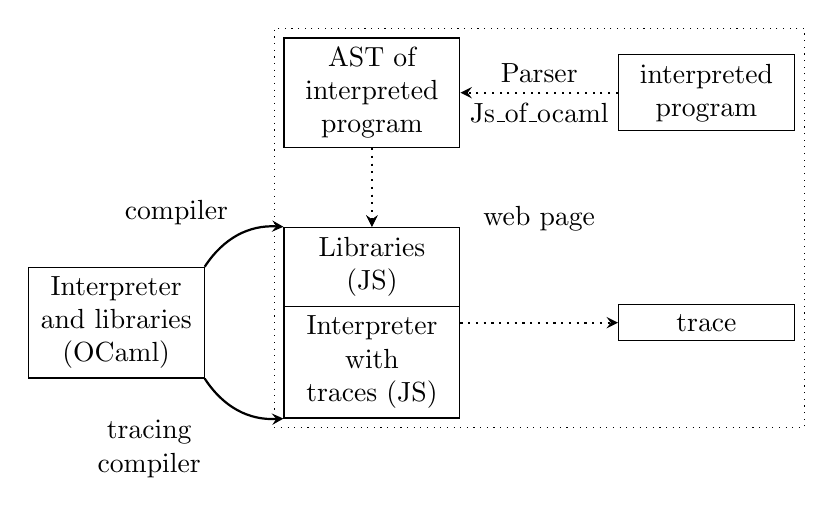
\begin{tikzpicture}[nodes = {align = center}]
    \node (focaml) [draw, text width=2cm] {Interpreter and libraries (OCaml)};

    \node (fjs) [draw, right = 1cm of focaml, text width=2cm, rectangle split,
    rectangle split parts=2, text centered] {Libraries (JS) \nodepart{second}
      Interpreter with traces (JS)};

    \node (ast) [draw, above = of fjs, text width=2cm] {AST of interpreted
      program};

    \node (source) [draw, right = 2cm of ast, text width=2cm, text centered]
    {interpreted program};

    \node [draw, dotted, fit=(fjs) (ast) (source)] {web page};

    \node (trace) [draw, right = 2cm of fjs, text width=2cm, text centered]
    {trace};

    \path[->,thick,>=stealth] (focaml.north
    east) edge[bend left] node[above left] {compiler} (fjs.north west) ;

    \path[->,thick,>=stealth] (focaml.south east) edge[bend right] node[below
    left] {\parbox{2cm}{\centering tracing compiler}} (fjs.south west);

    \path[->,thick,dotted,>=stealth] (source) edge node [above] {Parser} node
    [below] {Js\_of\_ocaml} (ast);

    \path[->,thick,dotted,>=stealth] (ast) edge (fjs);

    \path[->,thick,dotted,>=stealth] (ast) edge (fjs);

    \path[->,thick,dotted,>=stealth] (fjs) edge (trace);
  \end{tikzpicture}
  
  \caption{Architecture of MLExplain}
  \label{fig:archi}
\end{figure*}

To interpret OCaml code, we first need to parse and type it. However, our
compiler does not allow us to use the standard library nor an external one. As
we do not need to trace the parsing nor the typing, we have been able to
separate totally the frontend from the interpreter itself and use another
compiler to compile it. Figure \ref{fig:archi} describes the architecture of
the whole application.

The frontend is compiled with \emph{js\_of\_ocaml}
\cite{DBLP:journals/spe/VouillonB14}, the compiler of the project \emph{Ocsigen}
\cite{balat:hal-00691710}. The largest part of the frontend is a module that
serializes the \emph{Typedtree} -- the typed AST of OCaml -- into a JavaScript
object compatible with the backend interpreter's own representation of the AST.
We use the OCaml compiler, namely the \texttt{compiler-libs} library, to do the
actual parsing and typing. We thus have the guarantee that the typed AST we get
is the same as the official OCaml compiler AST.

Unfortunately, we cannot directly use the typed AST, as \emph{js\_of\_ocaml}
takes OCaml bytecode as input, which does not include sufficient information
such as the names of constructors. After parsing and typing, we thus navigate
the AST and call JavaScript functions that create the data in the expected format.

\subsection{Compiler limitations}

As stated before, the backend of our interpreter is written in a purely
functional strict subset of OCaml. As a consequence, it was necessary to encode
some features, such as exceptions. To this end, we use a monadic approach and
rely on \texttt{ppx} extensions to simplify the syntax.

As an example, consider the \texttt{option} monad, whose main operator is
defined as follows.

\begin{verbatim}
let bind_option opt f = match opt with
| Some value -> f value
| None -> None
\end{verbatim}

To use this operator, one would need to write the following.
\begin{verbatim}
bind_option
  (function_that_could_fail 0)
  (fun a -> continuation a)
\end{verbatim}
Such code can become difficult to read, especially when one is chaining several
functions.

The use of \texttt{ppx} lets us write the much simpler code, which is
transformed to the previous version during parsing.
\begin{verbatim}
let%some a = function_that_could_fail 0 in
continuation a
\end{verbatim}

\subsection{Web interface changes}

The data structures manipulated by MLExplain are very different from those
manipulated by JSExplain since they don't interpret the same language. We thus
had to modify the web interface so that it can recognize the different syntactic
elements of OCaml and pretty print them correctly as well as OCaml values.

Fortunately the web interface is very simple. It is composed of some auxiliary
JavaScript files, the main JavaScript file -- \texttt{navig-driver.js} --
containing the logic of the application and the corresponding HTML page. The
only modified file is \texttt{navig-driver.js}. The resulting tool can be tested
online.\footnote{\url{https://docteur-lalla.github.io/mlexplain/branch/master/driver.html}}

\section{Statistics}

We give some statistics about the project in Figure~\ref{fig:statistics}. As can
be seen, the largest part of the code is the frontend, in particular the
conversion from OCaml's AST to our format. The interpreter is quite short,
because the execution of OCaml is actually very simple. Note that we support all
of OCaml, with the exception of objects.

\begin{figure}[hb]
  \begin{tabular}{| c | c | c | c |}
    \hline
    & Comments & Code & Bind calls \\
    \hline
    Interpreter & 164 & 394 & 62 \\
    Primitives & 31 & 35 & 0 \\
    Execution context & 22 & 13 & 0 \\
    Frontend & 41 & 542 & 0 \\
    Syntax definition & 17 & 65 & 0 \\
    Auxiliary files & 72 & 232 & 2 \\
    \hline
    Total (no .mli) & 392 & 1621 & 70 \\
    Total (with .mli) & 401 & 1636 & 70 \\
    \hline
  \end{tabular}

  \centering
  \caption{Statistics about the project's code}
  \label{fig:statistics}
\end{figure}

\section{Conclusion}
We have shown how JSExplain can be easily adapted to other programming language,
in this case OCaml. Most of the complexity of OCaml being its typing, writing
the interpreter was quite straightforward. As future work, we plan to extend the
subset of OCaml supported by our compiler, to be able to directly use the
standard library when writing interpreters.

\bibliographystyle{plain}
\bibliography{biblio}

\end{document}
